\chapter{Inmunidad innata e inflamación}\label{ch:b3:innate-immunity}

Una astilla bajo la piel introduce diez mil bacterias que se duplicarán
cada media hora. En cuestión de minutos los vasos de alrededor se dilatan
y dejan escapar plasma; en una hora los primeros \omterm{def:b3:innate-immunity:innate}{neutrófilos} se han
escurrido fuera de la sangre y reptan hacia los intrusos siguiendo un
rastro químico; en un día el sitio está rojo, caliente, hinchado y
doloroso --- los cuatro signos de la \omterm{def:b3:innate-immunity:inflammation}{inflamación} que enumeró Celso hace
dos mil años --- y las bacterias están muertas, devoradas vivas por
células que las reconocieron como ajenas sin haberlas visto nunca antes.
Esto es la \omterm{def:b3:innate-immunity:innate}{inmunidad innata}: la defensa que tiene todo animal, lista
antes de la infección, codificada en el genoma en lugar de aprendida. Es
rápida, es la que mata a la mayoría de los invasores, y es la que le dice
a la inmunidad aprendida, más lenta, del capítulo siguiente que hay algo
que aprender. Sus excesos --- el choque séptico, la \omterm{def:b3:innate-immunity:inflammation}{inflamación} crónica,
las fiebres de las enfermedades autoinflamatorias --- son tan
instructivos como sus éxitos.

\section{Capas y células}

\begin{definition}[Inmunidad innata]\label{def:b3:innate-immunity:innate}
\index{inmunidad innata}\index{neutrófilo}\index{macrófago}\index{célula dendrítica}\index{linfocito citolítico natural}\index{barrera}
La \emph{inmunidad innata} es el conjunto de defensas presentes antes de
cualquier exposición, codificadas por genes de la línea germinal que no
se reordenan, que reconocen rasgos conservados de los microbios y no
individuos concretos, que actúan en minutos u horas y que (con matices)
carecen de memoria. Su primera capa son las \emph{barreras}: la queratina
de la piel, el moco y los \omterm{def:b3:cytoskeleton-motility:cilia}{cilios} de las vías respiratorias, el ácido del
estómago, el arrastre de la orina y de las lágrimas, la enzima lisozima
que corta el \omterm{def:b3:bacteriology:envelope}{peptidoglicano}, los \emph{péptidos antimicrobianos}
(defensinas, catelicidinas) que perforan las membranas microbianas y el
\omterm{def:b3:microbiomes:symbiosis}{microbioma} comensal que ocupa los nichos (\cref{ch:b3:microbiomes}). Sus
células, todas del linaje mieloide salvo la última: los
\emph{neutrófilos}, el \qty{60}{\%} de los leucocitos de la sangre, de
los que se fabrican $10^{11}$ al día y que viven un día, los primeros en
llegar y los principales verdugos de bacterias; los \emph{macrófagos},
residentes longevos de todos los tejidos (las células de Kupffer del
hígado, la microglía del cerebro, los macrófagos alveolares del pulmón)
que comen, limpian y dan la alarma; las \emph{células dendríticas}, que
muestrean los tejidos y llevan lo que encuentran a los ganglios
linfáticos; los mastocitos, los basófilos y los eosinófilos, armados
contra los parásitos y responsables de la alergia; y los
\emph{linfocitos citolíticos naturales} (NK), linfocitos que matan a
primera vista a las células infectadas o transformadas.
\end{definition}

\begin{proof}[Evidencia]
Metchnikoff (1882), en Mesina, clavó una espina de rosa en una larva
transparente de estrella de mar y vio, a la mañana siguiente, células
móviles apiñadas a su alrededor; había visto a esas mismas células
engullir partículas de alimento y granos de colorante, y propuso que
engullían también microbios --- los \emph{fagocitos}, agentes de una
defensa del hospedador que rastreó luego en todos los animales que
encontró, de las amebas al hombre. Compartió el premio Nobel de 1908 con
Ehrlich, cuyos anticuerpos representaban la visión opuesta, la humoral;
ambos tenían razón, y un siglo después se demostró que las dos mitades de
la inmunidad son un solo sistema, con la innata instruyendo a la
adaptativa.
\end{proof}

\begin{omfigure}
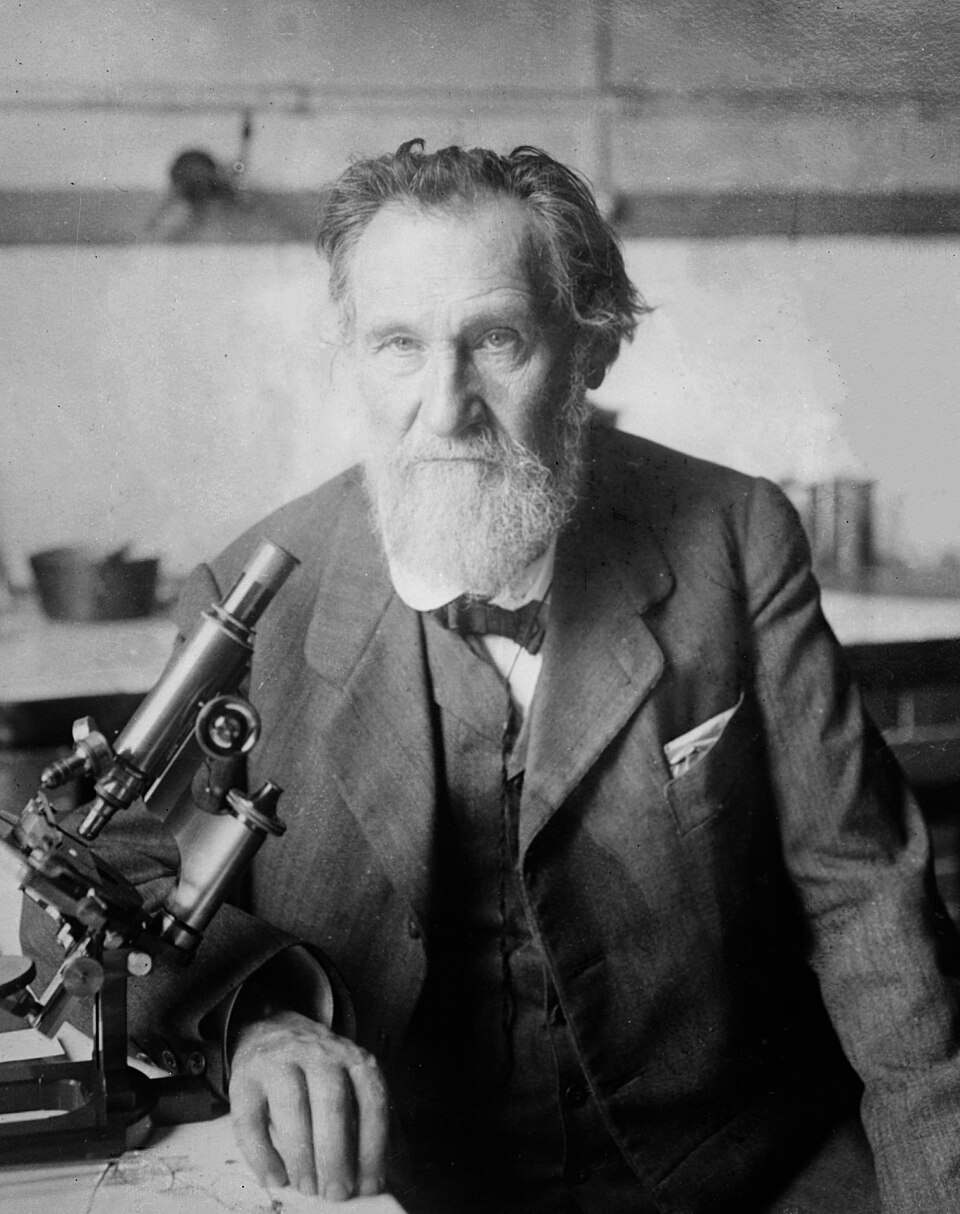
\includegraphics[width=0.30\linewidth]{images/book5/metchnikoff.jpg}\hspace{0.04\linewidth}
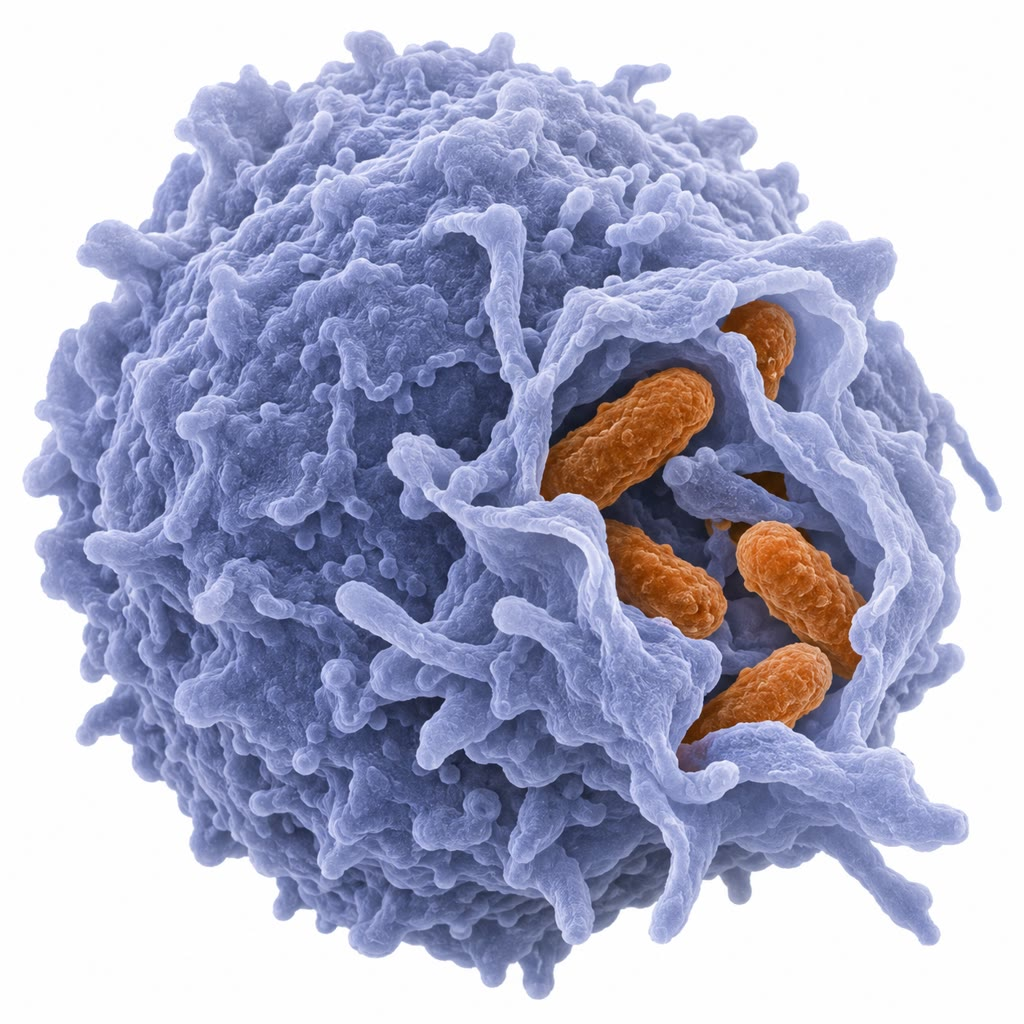
\includegraphics[width=0.30\linewidth]{images/book5/ai/b5-15-neutrophil-phagocytosis.jpg}\hspace{0.04\linewidth}
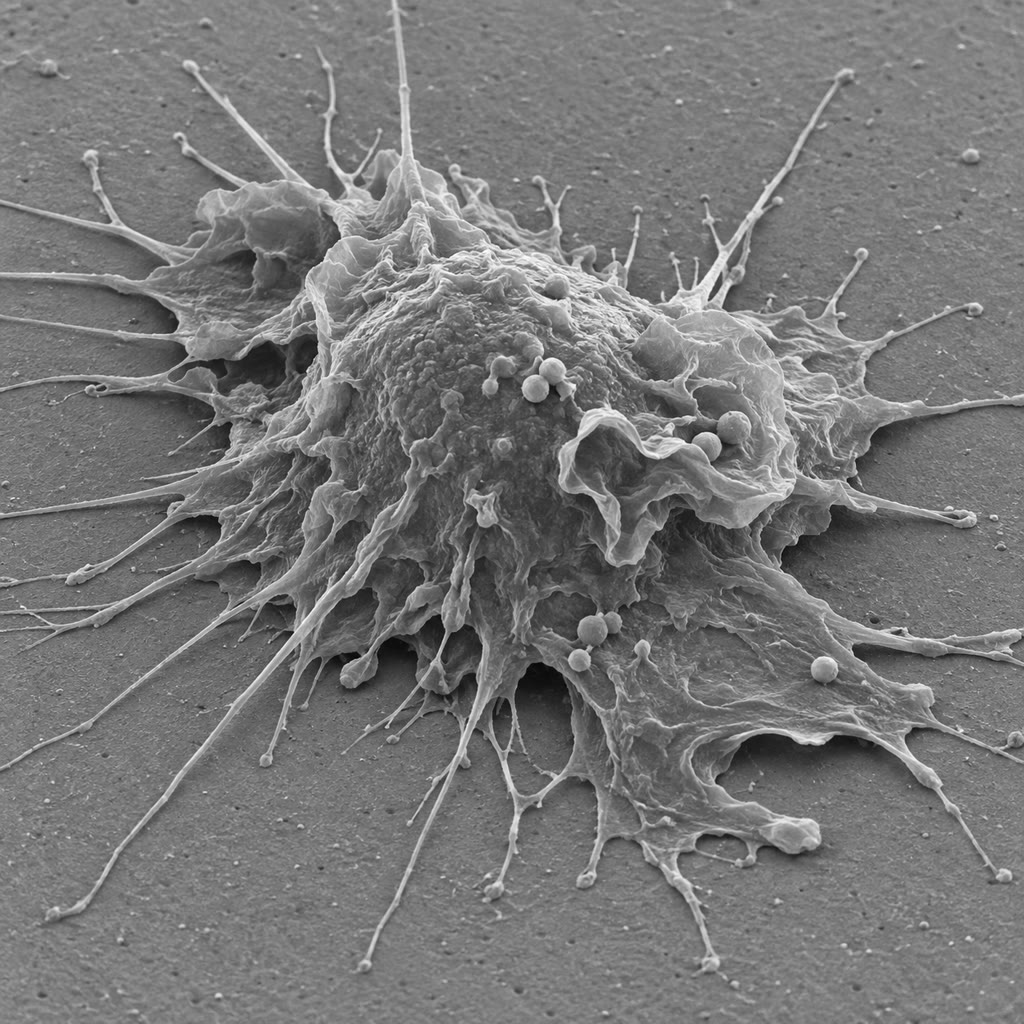
\includegraphics[width=0.30\linewidth]{images/book5/ai/b5-15-macrophage.jpg}

{\small Élie Metchnikoff, que vio cómo los fagocitos se agolpaban en
torno a una espina en una larva de estrella de mar y fundó la inmunología
celular (Biblioteca del Congreso, dominio público). Centro: un \omterm{def:b3:innate-immunity:innate}{neutrófilo}
engullendo bacterias. Derecha: un \omterm{def:b3:innate-immunity:innate}{macrófago} extendiendo sus membranas
ondulantes sobre una superficie.}
\end{omfigure}

\section{Reconocer al enemigo}

\begin{definition}[Reconocimiento de patrones]\label{def:b3:innate-immunity:prr}
\index{receptor de reconocimiento de patrones}\index{patrón molecular asociado a patógenos}\index{receptor de tipo Toll}\index{patrón molecular asociado a daño}\index{inflamasoma}
Las células innatas reconocen \emph{patrones moleculares asociados a
patógenos} (PAMP): moléculas comunes a clases enteras de microbios,
esenciales para ellos y ausentes del hospedador --- el \omterm{def:b3:bacteriology:envelope}{lipopolisacárido}
de las paredes \omterm{def:b3:bacteriology:envelope}{gramnegativas}, el \omterm{def:b3:bacteriology:envelope}{peptidoglicano} y el ácido lipoteicoico
de las \omterm{def:b3:bacteriology:envelope}{grampositivas}, la flagelina, los $\beta$-glucanos de los hongos,
el ARN de doble hebra, el ARN sin caperuza 5$'$, el ADN con \omterm{def:b3:chromatin-epigenetics:methylation}{CpG} sin
metilar, el ADN en el citosol. Los receptores son \emph{receptores de
reconocimiento de patrones} (PRR), unas pocas decenas en total,
codificados cada uno por un gen: los \emph{receptores de tipo Toll} (TLR)
de la superficie y de los \omterm{def:b3:membrane-traffic:endocytosis}{endosomas} (TLR4 para el \omterm{def:b3:bacteriology:envelope}{lipopolisacárido}, TLR5
para la flagelina, TLR3 para el ARN de doble hebra, TLR9 para el ADN con
\omterm{def:b3:chromatin-epigenetics:methylation}{CpG}); las proteínas NOD citosólicas para los fragmentos de
\omterm{def:b3:bacteriology:envelope}{peptidoglicano}, RIG-I para el ARN vírico, cGAS--STING para el ADN
citosólico; las lectinas de tipo C para los azúcares fúngicos. Esos
mismos receptores, u otros de las mismas familias, reconocen los
\emph{patrones moleculares asociados a daño} (DAMP) que liberan las
células lesionadas --- ATP, ácido úrico, la proteína nuclear HMGB1, ADN
mitocondrial ---, de modo que una lesión estéril también inflama. La
unión activa el factor de transcripción NF-$\kappa$B y los factores
reguladores del interferón, que en menos de una hora encienden \omterm{def:b3:innate-immunity:inflammation}{citocinas},
\omterm{def:b3:innate-immunity:inflammation}{quimiocinas}, moléculas de adhesión y genes antimicrobianos; y un
subconjunto de los sensores citosólicos ensambla el
\emph{inflamasoma}, una plataforma que activa la caspasa-1 para cortar la
interleucina-1$\beta$ y darle su forma activa y para desencadenar la
muerte inflamatoria llamada \omterm{def:b3:cell-cycle-apoptosis:other}{piroptosis}
(\cref{ch:b3:cell-cycle-apoptosis}).
\end{definition}

\begin{proof}[Evidencia]
Janeway propuso en 1989 que el sistema inmunitario adaptativo no responde
al antígeno solo, sino que necesita una señal de receptores innatos que
hayan reconocido patrones microbianos --- la explicación de por qué las
vacunas necesitan adyuvantes, ``el sucio secretillo del inmunólogo''.
Hoffmann (1996) descubrió que las \emph{Drosophila} sin el receptor Toll,
conocido por su papel en el patrón embrionario, no podían montar una
respuesta antifúngica y morían cubiertas de moho; Beutler (1998) localizó
la resistencia al \omterm{def:b3:bacteriology:envelope}{lipopolisacárido} de una cepa de ratón, que sobrevivía a
dosis de endotoxina letales para otras y no lograba eliminar las
infecciones \omterm{def:b3:bacteriology:envelope}{gramnegativas}, en una mutación del homólogo de mamífero TLR4.
El receptor de la endotoxina, buscado durante cincuenta años, era un
Toll.
\end{proof}

\begin{omfigure}
\begin{tikzpicture}[every node/.style={font=\scriptsize}, >=stealth]
  % membrane
  \draw[very thick, omDef] (0,3.0) -- (11.5,3.0); \draw[very thick, omDef] (0,2.7) -- (11.5,2.7);
  \node[above] at (0.5,3.05) {exterior}; \node[below] at (0.5,2.65) {citosol};
  % TLR4 with LPS
  \draw[thick, fill=omProp!35] (2.2,2.4) rectangle (2.6,3.9); \draw[thick, fill=omProp!35] (2.9,2.4) rectangle (3.3,3.9);
  \fill[omThm] (2.75,4.1) circle (0.14); \node[above] at (2.75,4.25) {LPS (un PAMP)};
  \node[right, align=left] at (3.4,3.5) {dímero de TLR4\\con MD2};
  % signalling
  \node[draw, thick, rounded corners, fill=omDef!20] (myd) at (2.75,1.7) {MyD88, quinasas};
  \node[draw, thick, rounded corners, fill=omDef!20] (nfkb) at (2.75,0.6) {NF-$\kappa$B liberado};
  \node[draw, thick, rounded corners, fill=omMeth!25, align=center] (genes) at (2.75,-0.8) {TNF, IL-1$\beta$, IL-6, IL-8;\\moléculas de adhesión; iNOS};
  \draw[->, thick] (2.75,2.4) -- (myd); \draw[->, thick] (myd) -- (nfkb); \draw[->, thick] (nfkb) -- (genes);
  \node[right, font=\tiny] at (3.3,1.2) {en menos de una hora};
  % cytosolic sensors
  \node[draw, thick, rounded corners, fill=omProp!25, align=center] (rig) at (6.9,1.9) {RIG-I: ARN vírico\\cGAS--STING: ADN citosólico};
  \node[draw, thick, rounded corners, fill=omMeth!25] (ifn) at (6.9,-0.2) {interferón de tipo I};
  \draw[->, thick] (rig) -- node[midway, right] {IRF3, IRF7} (ifn);
  \node[draw, thick, rounded corners, fill=omThm!20, align=center] (nlrp) at (10.9,1.9) {inflamasoma NLRP3:\\cristales, ATP, poros};
  \node[draw, thick, rounded corners, fill=omMeth!25, align=center] (il1) at (10.9,-0.8) {caspasa-1: IL-1$\beta$\\liberada; piroptosis};
  \draw[->, thick] (nlrp) -- (il1);
  \draw[->, thick, dashed] (genes.south) -- ++(0,-0.5) -| (il1.south) node[pos=0.25, below, font=\tiny] {la vía TLR aporta la pro-IL-1$\beta$};
\end{tikzpicture}

{\small Tres brazos del reconocimiento de patrones. Un \omterm{def:b3:innate-immunity:prr}{receptor de tipo
Toll} de superficie unido por el \omterm{def:b3:bacteriology:envelope}{lipopolisacárido} señaliza a través de
NF-$\kappa$B hacia las \omterm{def:b3:innate-immunity:inflammation}{citocinas} inflamatorias; los sensores citosólicos
de ácido nucleico vírico inducen interferón; y el \omterm{def:b3:innate-immunity:prr}{inflamasoma} convierte
el precursor almacenado de la interleucina-1 en la \omterm{def:b3:innate-immunity:inflammation}{citocina} activa.}
\end{omfigure}

\begin{definition}[Complemento]\label{def:b3:innate-immunity:complement}
\index{complemento}\index{convertasa de C3}\index{opsonización}\index{complejo de ataque a la membrana}\index{anafilotoxina}
El \emph{complemento} es un sistema de unas treinta proteínas
plasmáticas, el \qty{10}{\%} de las globulinas del suero, que marca y
destruye microbios mediante una cascada de activaciones proteolíticas.
Tres vías convergen en el corte de la proteína central, C3: la vía
\emph{clásica}, que inicia C1q al unirse a anticuerpos sobre una
superficie (o a la \omterm{prop:b3:innate-immunity:systemic}{proteína C reactiva}, o a células apoptóticas); la vía
\emph{de las lectinas}, que inicia la lectina de unión a manosa al
reconocer azúcares microbianos; y la vía \emph{alternativa}, en la que C3
se hidroliza espontáneamente a baja velocidad y el C3b resultante se pega
a cualquier superficie que encuentre. Cada vía construye una
\emph{convertasa de C3}, una enzima que corta más C3; el C3b que deposita
covalentemente sobre la superficie construye a su vez más convertasa ---
un bucle de amplificación ---, de modo que una bacteria queda recubierta
de millones de C3b en cuestión de minutos. El C3b es una
\emph{opsonina}: los fagocitos llevan receptores para él y se comen lo
que recubre. Los fragmentos pequeños C3a y C5a son \emph{anafilotoxinas}
que dilatan los vasos, atraen \omterm{def:b3:innate-immunity:innate}{neutrófilos} y activan mastocitos. Y C5b
ensambla C6--C9 en el \emph{complejo de ataque a la membrana}, un poro de
\qty{10}{nm} que lisa bacterias \omterm{def:b3:bacteriology:envelope}{gramnegativas} y \omterm{def:b3:virology:virus}{virus} con envoltura. Las
células del hospedador se salvan porque llevan reguladores --- el factor
H, CD55, CD59 --- que desmontan la convertasa y bloquean el poro en sus
propias superficies; los microbios, que carecen de ellos, son consumidos
por el bucle.
\end{definition}

\begin{theorem}[El bucle del complemento como discriminador cinético]\label{thm:b3:innate-immunity:complement}
\index{complemento!bucle de amplificación}
Sea $B(t)$ el número de moléculas de C3b depositadas sobre una
superficie. El C3b se deposita a una pequeña velocidad constante $k_{0}$
por el goteo del C3, y cada C3b depositado construye convertasa que
deposita más a velocidad $a$ por C3b y segundo, mientras que los
reguladores (del hospedador) y la desintegración retiran actividad de
convertasa a velocidad $d$ por C3b y segundo:
\[
\frac{\mathrm{d}B}{\mathrm{d}t} = k_{0} + (a - d)\,B .
\]
En una superficie donde $a > d$ --- un microbio, sin reguladores ---,
$B(t) = \bigl[k_{0}/(a-d)\bigr]\bigl(e^{(a-d)t} - 1\bigr)$ crece
exponencialmente con constante de tiempo $1/(a - d)$; en una superficie
del hospedador, donde $d > a$, $B$ se acerca al pequeño valor
estacionario $k_{0}/(d - a)$. Las mismas moléculas, a las mismas
concentraciones, depositan un millón de C3b sobre una bacteria en unos
minutos y unas pocas decenas sobre la célula de al lado: la distinción
entre lo propio y lo ajeno no la hace el reconocimiento, sino el signo de
$a - d$.
\end{theorem}
\begin{proof}
La ecuación es lineal de coeficientes constantes. Para $a \ne d$ el punto
fijo es $B^{*} = -k_{0}/(a-d)$; escribiendo $B = B^{*} + u$,
$\mathrm{d}u/\mathrm{d}t = (a-d)u$, luego $u = u_{0}e^{(a-d)t}$ y, con
$B(0) = 0$, $B(t) = \bigl[k_{0}/(a-d)\bigr](e^{(a-d)t} - 1)$. Para
$a > d$ esto crece sin límite (hasta que se agotan el C3 o la
superficie); para $a < d$ la exponencial decae y $B \to k_{0}/(d-a) > 0$.
Con $k_{0} = 1$ por segundo y $a - d = \qty{0.1}{s^{-1}}$ en una
bacteria, $B(\qty{2}{min})
= 10(e^{12} - 1) \approx 1.6\times 10^{6}$; con $d - a =
\qty{0.1}{s^{-1}}$ en una célula del hospedador, $B^{*} = 10$.
\end{proof}

\begin{omfigure}
\begin{tikzpicture}
\begin{axis}[
  width=0.66\linewidth, height=5.6cm,
  axis x line=bottom, axis y line=left,
  xmin=0, xmax=150, ymin=1, ymax=1e7, ymode=log,
  xlabel={segundos}, ylabel={C3b depositado},
  xlabel style={font=\small, at={(axis description cs:0.5,-0.12)}, anchor=north}, ylabel style={font=\small},
  tick label style={font=\small}, xtick={0,30,60,90,120,150},
  clip=false,
]
\addplot[very thick, omThm, domain=1:150, samples=80] {10*(exp(0.1*x)-1)};
\addplot[very thick, omDef, domain=1:150, samples=80] {10*(1-exp(-0.1*x))};
\node[font=\scriptsize, omThm, anchor=east] at (axis cs:100,2e5) {microbio: $a > d$, exponencial};
\node[font=\scriptsize, omDef, anchor=south west] at (axis cs:60,14) {célula del hospedador: $d > a$, satura en $k_{0}/(d-a)$};
\end{axis}
\end{tikzpicture}

{\small El bucle del \omterm{def:b3:innate-immunity:complement}{complemento} sobre dos superficies con $k_{0} = 1$
por segundo y $|a - d| = \qty{0.1}{s^{-1}}$: sobre un microbio sin
reguladores el C3b crece exponencialmente y llega al millón en dos
minutos; sobre una célula del hospedador con reguladores se estabiliza en
diez.}
\end{omfigure}

\begin{omfigure}
\begin{tikzpicture}[every node/.style={font=\scriptsize}, >=stealth]
  \node[draw, thick, rounded corners, fill=omDef!20, align=center] (cl) at (-4.2,3.0) {clásica:\\C1q sobre anticuerpo\\o proteína C reactiva};
  \node[draw, thick, rounded corners, fill=omDef!20, align=center] (le) at (0,3.0) {de las lectinas:\\lectina de unión a manosa\\sobre azúcares microbianos};
  \node[draw, thick, rounded corners, fill=omDef!20, align=center] (al) at (4.2,3.0) {alternativa:\\goteo espontáneo de C3,\\C3b sobre cualquier superficie};
  \node[draw, thick, rounded corners, fill=omProp!35, minimum width=3cm] (conv) at (0,1.2) {convertasa de C3};
  \node[draw, thick, rounded corners, fill=omThm!25, align=center] (c3b) at (0,-0.4) {C3 $\to$ C3b (en la superficie) $+$ C3a};
  \draw[->, thick] (cl) -- (conv); \draw[->, thick] (le) -- (conv); \draw[->, thick] (al) -- (conv);
  \draw[->, thick] (conv) -- (c3b);
  \draw[->, very thick, omThm] (c3b.east) .. controls (3.2,-0.4) and (3.2,1.2) .. (conv.east) node[pos=0.5, right, align=left] {bucle de amplificación:\\el C3b construye más convertasa};
  \node[draw, thick, rounded corners, fill=omMeth!25, align=center] (ops) at (-4.4,-2.2) {opsonización:\\los fagocitos comen\\lo que el C3b recubre};
  \node[draw, thick, rounded corners, fill=omMeth!25, align=center] (ana) at (0,-2.2) {C3a, C5a:\\los vasos se dilatan y se reclutan\\neutrófilos y mastocitos};
  \node[draw, thick, rounded corners, fill=omMeth!25, align=center] (mac) at (4.4,-2.2) {C5b--C9:\\complejo de ataque a la membrana,\\lisis};
  \draw[->, thick] (c3b) -- (ops); \draw[->, thick] (c3b) -- (ana); \draw[->, thick] (c3b) -- (mac);
  \node[draw, thick, rounded corners, fill=gray!15, align=center] (reg) at (-4.4,1.2) {reguladores del hospedador:\\factor H, CD55, CD59};
  \draw[-|, thick, gray!60!black] (reg) -- (conv);
\end{tikzpicture}

{\small El \omterm{def:b3:innate-immunity:complement}{complemento}. Tres rutas construyen una \omterm{def:b3:innate-immunity:complement}{convertasa de C3}; el
C3b que esta deposita construye más (el bucle del teorema), y el C3b
depositado opsoniza, los fragmentos inflaman y el complejo terminal lisa.
Las células del hospedador llevan reguladores que cortan el bucle (y,
con CD59, bloquean el poro) en sus propias membranas.}
\end{omfigure}

\section{La inflamación}

\begin{definition}[Inflamación aguda]\label{def:b3:innate-immunity:inflammation}
\index{inflamación}\index{citocina}\index{quimiocina}\index{extravasación}\index{selectina}\index{integrina}
La \emph{inflamación} es la respuesta de un tejido vascularizado a una
lesión o a una infección, orquestada por \emph{citocinas} --- las
pequeñas proteínas de señalización de las células inmunitarias, aquí
sobre todo el TNF, la interleucina-1 y la interleucina-6 de los
\omterm{def:b3:innate-immunity:innate}{macrófagos} activados --- y por \emph{quimiocinas}, las citocinas que
dirigen la migración. Sus pasos explican los signos de Celso. La
histamina de los mastocitos, el óxido nítrico y las prostaglandinas
dilatan las arteriolas: el \emph{enrojecimiento} y el \emph{calor}. El
endotelio de las vénulas se contrae y deja escapar plasma, cuyas
proteínas --- \omterm{def:b3:innate-immunity:complement}{complemento}, anticuerpos, factores de coagulación ---
inundan el tejido: la \emph{hinchazón}. La bradicinina y la
prostaglandina E$_{2}$ sensibilizan las terminaciones nerviosas: el
\emph{dolor}. Y los leucocitos llegan por \emph{extravasación}: el TNF y
la interleucina-1 hacen que el endotelio muestre \emph{selectinas},
sobre las que los \omterm{def:b3:innate-immunity:innate}{neutrófilos} que pasan se enganchan y ruedan; las
quimiocinas (la interleucina-8) de la superficie endotelial activan las
\emph{integrinas} de los \omterm{def:b3:innate-immunity:innate}{neutrófilos}, que se unen con fuerza a las
moléculas de adhesión endoteliales y detienen la célula; y el \omterm{def:b3:innate-immunity:innate}{neutrófilo}
se cuela entre las células endoteliales y sigue el gradiente de
quimiocina hacia el tejido --- toda la secuencia en unos minutos, y hasta
un millón de células por hora hacia un sitio infectado.
\end{definition}

\begin{omfigure}
\begin{tikzpicture}[every node/.style={font=\scriptsize}, >=stealth]
  % vessel wall
  \fill[omThm!10] (0,0) rectangle (12,2.3); \node[left, omThm!70!black, anchor=north east] at (12,2.25) {sangre, fluyendo $\rightarrow$};
  \foreach \x in {0,1.5,3,4.5,6,7.5,9,10.5} \draw[thick, fill=omDef!30] (\x,-0.05) rectangle (\x+1.45,0.35);
  \node[right] at (0.1,-0.35) {endotelio};
  \fill[omMeth!8] (0,-1.7) rectangle (12,-0.45); \node[right, omMeth!60!black] at (0.1,-1.55) {tejido};
  % bacteria and chemokine gradient
  \foreach \p in {(10.6,-1.1),(11.0,-0.9),(11.3,-1.2)} \fill[omProp] \p ellipse (0.14 and 0.07);
  \node[below, omProp] at (11.0,-1.35) {bacterias};
  \node[below, font=\tiny] at (8.0,-0.5) {gradiente de quimiocina $\rightarrow$};
  % neutrophils in sequence
  \draw[thick, fill=white] (1.2,1.1) circle (0.3); \node[above] at (1.2,1.45) {1. fluyendo};
  \draw[thick, fill=white] (3.4,0.68) circle (0.3); \node[above] at (3.4,1.05) {2. rodando sobre selectinas};
  \draw[omThm, thick] (3.1,0.45) -- (3.05,0.35); \draw[omThm, thick] (3.4,0.38) -- (3.4,0.35); \draw[omThm, thick] (3.7,0.45) -- (3.75,0.35);
  \draw[thick, fill=white] (6.0,0.62) ellipse (0.38 and 0.26); \node[above, align=center] at (6.0,0.95) {3. adhesión firme\\(integrinas)};
  \draw[thick, fill=white] (8.25,0.18) ellipse (0.2 and 0.42); \node[above, align=center] at (8.4,0.95) {4. colándose\\entre las células};
  \draw[thick, fill=white] (9.6,-1.0) circle (0.3); \node[left] at (9.25,-1.0) {5. reptando hacia el foco};
  \draw[->, thick, gray] (1.5,1.05) -- (3.0,0.8); \draw[->, thick, gray] (3.7,0.68) -- (5.6,0.62); \draw[->, thick, gray] (6.4,0.5) -- (8.0,0.4); \draw[->, thick, gray] (8.3,-0.3) -- (9.3,-0.8);
  % TNF label
  \node[below, align=center, font=\tiny] at (4.0,-1.75) {el TNF y la IL-1 de los macrófagos del tejido hacen que el endotelio\\muestre las selectinas y las moléculas de adhesión que atrapan a los neutrófilos};
\end{tikzpicture}

{\small La \omterm{def:b3:innate-immunity:inflammation}{extravasación}. Las \omterm{def:b3:innate-immunity:inflammation}{citocinas} de los \omterm{def:b3:innate-immunity:innate}{macrófagos} del tejido
vuelven pegajosa la pared de la vénula; un \omterm{def:b3:innate-immunity:innate}{neutrófilo} que pasa se engancha
a las \omterm{def:b3:innate-immunity:inflammation}{selectinas} y rueda, sus \omterm{def:b3:innate-immunity:inflammation}{integrinas} lo detienen, se cuela entre las
células endoteliales y sigue el gradiente de \omterm{def:b3:innate-immunity:inflammation}{quimiocina} hasta las
bacterias.}
\end{omfigure}

\begin{proposition}[Fiebre, fase aguda y resolución]\label{prop:b3:innate-immunity:systemic}
\index{fiebre}\index{respuesta de fase aguda}\index{proteína C reactiva}\index{resolución de la inflamación}
La interleucina-1, el TNF y la interleucina-6 actúan también a
distancia. En el hipotálamo inducen prostaglandina E$_{2}$, que sube el
punto de ajuste de la temperatura corporal: la \emph{fiebre}, que frena a
muchas bacterias, acelera las reacciones de las propias células
inmunitarias y cuesta alrededor de un \qty{12}{\%} más de metabolismo por
grado. En el hígado inducen las \emph{proteínas de fase aguda} --- la
\omterm{prop:b3:innate-immunity:systemic}{proteína C reactiva}, que une la fosfocolina bacteriana, activa el
\omterm{def:b3:innate-immunity:complement}{complemento} y sube mil veces en dos días, la medida de la \omterm{def:b3:innate-immunity:inflammation}{inflamación} que
usa el clínico; el fibrinógeno; la lectina de unión a manosa; y la
hepcidina, que encierra el hierro lejos de los microbios que lo
necesitan. En la médula liberan \omterm{def:b3:innate-immunity:innate}{neutrófilos} y aceleran su producción. La
\omterm{def:b3:innate-immunity:inflammation}{inflamación} está hecha para terminar: a medida que se elimina el
estímulo, los mediadores lipídicos pasan de las prostaglandinas a las
lipoxinas y las resolvinas, los \omterm{def:b3:innate-immunity:innate}{neutrófilos} mueren por \omterm{def:b3:cell-cycle-apoptosis:apoptosis}{apoptosis} y los
comen los \omterm{def:b3:innate-immunity:innate}{macrófagos}, que pasan entonces a un programa de reparación y
secretan factores de crecimiento e interleucina-10 --- la
\emph{resolución}. Cuando el estímulo persiste (un bacilo tuberculoso al
que no se puede matar, un cristal, un autoantígeno), la respuesta se
vuelve crónica: los \omterm{def:b3:innate-immunity:innate}{macrófagos} amurallan el sitio en un granuloma, los
fibroblastos depositan cicatriz y el tejido queda destruido por su propia
defensa.
\end{proposition}

\begin{example}[La sepsis]\label{ex:b3:innate-immunity:sepsis}
Una \omterm{def:b3:innate-immunity:inflammation}{inflamación} confinada a una astilla es una cura; esas mismas
reacciones por todo el cuerpo son una catástrofe. Cuando las bacterias o
su \omterm{def:b3:bacteriology:envelope}{lipopolisacárido} llegan a la sangre en cantidad, los \omterm{def:b3:innate-immunity:innate}{macrófagos} de
todas partes liberan TNF e interleucina-1 a la vez: todos los vasos se
dilatan y dejan escapar plasma, la presión arterial se desploma, la
coagulación se activa en diez mil capilares y consume los factores de
coagulación, y los órganos, privados de perfusión, fallan --- el
\emph{choque séptico}, que mata a entre una cuarta parte y la mitad de
aquellos a los que golpea, unos once millones de personas al año. Unos
pocos microgramos de \omterm{def:b3:bacteriology:envelope}{lipopolisacárido} inyectados en un voluntario
producen fiebre, escalofríos y una caída de la presión arterial en menos
de dos horas; un ratón sin TLR4 se sacude una dosis cien veces letal. La
enfermedad es la respuesta del hospedador, y los \omterm{def:b3:bacteriology:antibiotics}{antibióticos} que matan a
las bacterias pueden empeorarla durante unas horas al liberar más
endotoxina.
\end{example}

\begin{omfigure}
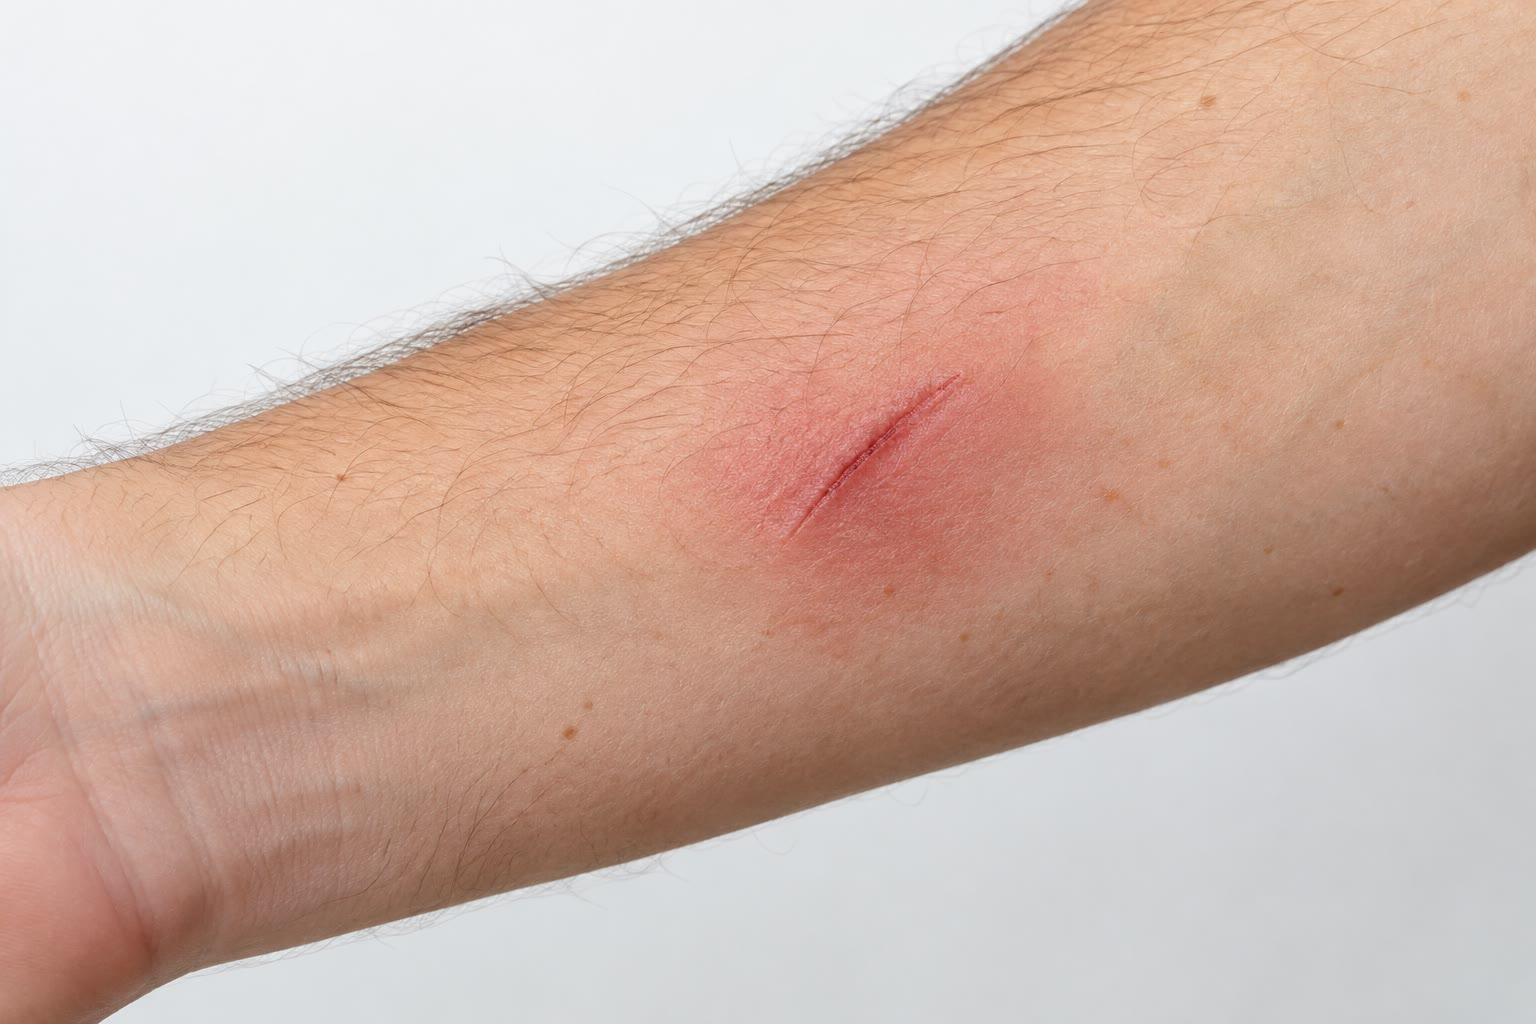
\includegraphics[width=0.52\linewidth]{images/book5/ai/b5-15-inflamed-skin.jpg}

{\small \omterm{def:b3:innate-immunity:inflammation}{Inflamación} aguda alrededor del arañazo de una espina:
enrojecimiento y calor por los vasos dilatados, hinchazón por el plasma
escapado y el dolor que mantiene quieto el miembro --- la respuesta local
que, generalizada a todo el cuerpo, es el choque séptico.}
\end{omfigure}

\section{Matar}

\begin{definition}[Fagocitosis y estallido respiratorio]\label{def:b3:innate-immunity:killing}
\index{fagocitosis}\index{estallido respiratorio}\index{NADPH-oxidasa}\index{trampa extracelular de neutrófilo}
Un fagocito une a su presa mediante receptores de opsoninas --- el C3b y
las regiones constantes de los anticuerpos --- o directamente mediante
receptores de patrones, la envuelve en membrana y cierra el
\emph{fagosoma}, que se fusiona con gránulos y \omterm{def:b3:membrane-traffic:endocytosis}{lisosomas}. La muerte llega
por varios medios a la vez. El \emph{estallido respiratorio}: la enzima
\emph{NADPH-oxidasa}, ensamblada en la membrana del fagosoma, bombea
electrones al oxígeno para producir superóxido, que pasa a peróxido de
hidrógeno, que la mieloperoxidasa convierte, con cloruro, en hipoclorito
--- lejía, a concentración milimolar dentro de un compartimento de un
micrómetro. Óxido nítrico de la NO-sintasa inducible, que con el
superóxido da peroxinitrito. Ácido, hasta pH~5. Lisozima, proteasas,
lactoferrina que priva de hierro a la presa y defensinas que la perforan.
Un \omterm{def:b3:innate-immunity:innate}{neutrófilo} que no puede comerse lo que encuentra --- una hifa de
hongo, un grumo --- puede expulsar su propia \omterm{def:b3:chromatin-epigenetics:nucleosome}{cromatina} como una red
pegajosa de ADN y proteínas de gránulo, una \emph{trampa extracelular de
\omterm{def:b3:innate-immunity:innate}{neutrófilo}}, y morir haciéndolo. Los niños que heredan una NADPH-oxidasa
defectuosa (la enfermedad granulomatosa crónica) sufren abscesos y
granulomas repetidos por bacterias y hongos que los fagocitos corrientes
matan sin dificultad: el estallido no es opcional.
\end{definition}

\begin{definition}[Linfocitos citolíticos naturales e interferón]\label{def:b3:innate-immunity:nk-ifn}
\index{linfocito citolítico natural!ausencia de lo propio}\index{interferón!de tipo I}\index{estado antivírico}
Los \omterm{def:b3:virology:virus}{virus} se esconden dentro de las células, donde el \omterm{def:b3:innate-immunity:complement}{complemento} y los
fagocitos no pueden alcanzarlos. Los \emph{\omterm{def:b3:innate-immunity:innate}{linfocitos citolíticos
naturales}} patrullan buscando células que han dejado de mostrar MHC de
clase~I --- la ``ausencia de lo propio'' de una célula cuyo ocupante
vírico o tumoral ha apagado la presentación de antígenos para escapar de
los linfocitos~T (\cref{ch:b3:adaptive-immunity}) --- y buscando
proteínas de estrés que las células infectadas y transformadas ponen en
su superficie; se suman los receptores inhibidores del MHC~I y los
receptores activadores de los ligandos de estrés, y la célula que
desequilibra el balance muere en minutos por la perforina y las
granzimas que se le inyectan, que disparan su \omterm{def:b3:cell-cycle-apoptosis:apoptosis}{apoptosis}. Los
\emph{interferones de tipo~I} ($\alpha$ y $\beta$) los fabrica cualquier
célula cuyo RIG-I o cuya cGAS haya detectado ácido nucleico vírico;
secretados, se unen a receptores de las células vecinas y, a través de la
vía JAK--STAT, inducen centenares de genes que ponen a esas células en un
\emph{estado \omterm{def:b3:virology:drugs}{antivírico}}: una quinasa que apaga la traducción cuando se
encuentra con ARN de doble hebra, una nucleasa que degrada ARN, proteínas
que bloquean la entrada y el ensamblaje víricos y más MHC~I para enseñar
a los linfocitos~T lo que hay dentro. La célula que fabricó el interferón
puede morir; sus vecinas quedan avisadas. El interferón lo descubrieron
Isaacs y Lindenmann (1957) como el factor del medio de células infectadas
por un \omterm{def:b3:virology:virus}{virus} que volvía resistentes a células frescas, y es la razón de
que una célula infectada por un \omterm{def:b3:virology:virus}{virus} resista a un segundo.
\end{definition}

\begin{method}[Medir la inflamación y la función de los fagocitos]\label{met:b3:innate-immunity:tests}
\index{proteína C reactiva!determinación}\index{prueba del nitroazul de tetrazolio}
A pie de cama: (1) la \emph{\omterm{prop:b3:innate-immunity:systemic}{proteína C reactiva}} del suero, por
inmunoensayo --- por debajo de \qty{5}{mg/L} en reposo, decenas en una
infección vírica, centenares en una sepsis bacteriana, y cayendo en
cuestión de días si el tratamiento es eficaz; (2) el recuento de
\omterm{def:b3:innate-immunity:innate}{neutrófilos}, elevado en la infección bacteriana, con formas inmaduras
liberadas pronto de la médula; (3) la velocidad de sedimentación
globular, un indicador lento del fibrinógeno. Para los fagocitos: (4) la
prueba del \emph{nitroazul de tetrazolio} o de la dihidrorrodamina, en la
que los \omterm{def:b3:innate-immunity:innate}{neutrófilos} estimulados in vitro reducen un colorante si su
\omterm{def:b3:innate-immunity:killing}{NADPH-oxidasa} funciona --- el diagnóstico de la enfermedad granulomatosa
crónica en una mañana; (5) un ensayo de quimiotaxis, que cuenta las
células que migran a través de un filtro hacia una \omterm{def:b3:innate-immunity:inflammation}{quimiocina}.
\end{method}

\section{De la innata a la adaptativa, y a lo largo de la vida}

\begin{proposition}[La decisión de la célula dendrítica]\label{prop:b3:innate-immunity:bridge}
\index{célula dendrítica!maduración}\index{coestimulación}\index{adyuvante}
La inmunidad adaptativa no se pone en marcha sola. Una \emph{\omterm{def:b3:innate-immunity:innate}{célula
dendrítica}} de un tejido se come lo que encuentra; si se disparan sus
receptores de patrones --- por un microbio o por un daño ---, madura:
deja de comer, migra por los linfáticos hasta el ganglio linfático que
drena la zona, muestra en moléculas del MHC los péptidos de lo que comió
y levanta moléculas \emph{coestimuladoras} (B7) y \omterm{def:b3:innate-immunity:inflammation}{citocinas} que le dicen
a un linfocito~T que reconozca el péptido que responda, y cómo
(\cref{ch:b3:adaptive-immunity}). Un linfocito~T que ve su péptido en una
\omterm{def:b3:innate-immunity:innate}{célula dendrítica} sin coestimulación queda apagado. El reconocimiento
innato decide así si un antígeno merece una respuesta, y las \omterm{def:b3:innate-immunity:inflammation}{citocinas}
que fabrica la \omterm{def:b3:innate-immunity:innate}{célula dendrítica} --- decididas por qué receptores de
patrones se dispararon --- deciden si la respuesta se dirige contra
\omterm{def:b3:virology:virus}{virus}, contra bacterias o contra gusanos. Un \emph{adyuvante} es un
ligando de receptores de patrones añadido a una vacuna para aportar esta
señal; el alumbre y las nanopartículas lipídicas de las vacunas modernas
funcionan disparándola.
\end{proposition}

\begin{remark}[La inmunidad innata en todas partes, y su memoria]\label{rem:b3:innate-immunity:everywhere}
Todo organismo pluricelular tiene \omterm{def:b3:innate-immunity:innate}{inmunidad innata}, y las plantas, los
hongos y los invertebrados no tienen ninguna otra. Las plantas reconocen
la flagelina y la quitina con receptores quinasa y montan una respuesta
en dos niveles (\cref{ch:b3:plant-molecular-physiology}); los insectos
tienen Toll y péptidos antimicrobianos; y hasta las bacterias tienen
\omterm{def:b3:genetic-engineering:tools}{enzimas de restricción} y \omterm{def:b3:genetic-engineering:crispr}{CRISPR} (\cref{ch:b3:genetic-engineering}). El
dogma de que la \omterm{def:b3:innate-immunity:innate}{inmunidad innata} no tiene memoria se ha ablandado: un
monocito que se ha encontrado con $\beta$-glucano o con la vacuna BCG
queda reprogramado epigenéticamente
(\cref{ch:b3:chromatin-epigenetics}) para responder con más fuerza a
microbios no emparentados durante meses --- la \emph{inmunidad
entrenada}, que explica por qué la BCG baja la mortalidad infantil por
infecciones distintas de la tuberculosis. Y el exceso del sistema es una
enfermedad de nuestro tiempo: la \omterm{def:b3:innate-immunity:inflammation}{inflamación} estéril que impulsan los
cristales de ácido úrico (la gota), los cristales de colesterol de la
pared arterial (la aterosclerosis), el \omterm{def:b3:structural-biology:amyloid}{amiloide} del cerebro y la
\omterm{def:b3:innate-immunity:inflammation}{inflamación} de bajo grado de la obesidad y de la vejez.
\end{remark}

\section{Ejercicios}

\begin{exercise}[$\star$]\label{exo:b3:innate-immunity:1}
Enumérense cuatro \omterm{def:b3:innate-immunity:innate}{barreras} y cinco tipos celulares de la \omterm{def:b3:innate-immunity:innate}{inmunidad
innata}, con una función de cada uno.
\end{exercise}

\begin{exercise}[$\star$]\label{exo:b3:innate-immunity:2}
¿Qué hace de una molécula un buen \omterm{def:b3:innate-immunity:prr}{patrón molecular asociado a patógenos}?
Dense tres ejemplos y el receptor de cada uno.
\end{exercise}

\begin{exercise}[$\star$]\label{exo:b3:innate-immunity:3}
Explíquese cada uno de los cuatro signos de Celso con un mediador y un
cambio vascular o nervioso.
\end{exercise}

\begin{exercise}[$\star$]\label{exo:b3:innate-immunity:4}
Nómbrense las tres vías del \omterm{def:b3:innate-immunity:complement}{complemento}, qué inicia cada una y los tres
resultados del corte del C3.
\end{exercise}

\begin{exercise}[$\star\star$]\label{exo:b3:innate-immunity:5}
En el modelo del \omterm{def:b3:innate-immunity:complement}{complemento} con $k_{0} = 2$ por segundo, $a =
\qty{0.15}{s^{-1}}$ y $d = \qty{0.05}{s^{-1}}$ en un microbio, ¿cuántos
C3b se depositan al cabo de \qty{60}{s}? ¿Y de \qty{90}{s}? En una célula
del hospedador con $a = 0.05$ y $d = 0.15$, ¿cuál es el estado
estacionario?
\end{exercise}

\begin{exercise}[$\star\star$]\label{exo:b3:innate-immunity:6}
Ordénense los sucesos de la \omterm{def:b3:innate-immunity:inflammation}{extravasación}, nómbrese la clase de molécula
de cada paso y predígase el fenotipo de un niño cuyos \omterm{def:b3:innate-immunity:innate}{neutrófilos} carecen
de \omterm{def:b3:innate-immunity:inflammation}{integrinas} $\beta_{2}$ (la deficiencia de adhesión leucocitaria).
\end{exercise}

\begin{exercise}[$\star\star$]\label{exo:b3:innate-immunity:7}
Los \omterm{def:b3:innate-immunity:innate}{neutrófilos} de un paciente no superan la prueba de la
dihidrorrodamina. ¿Cuál es el diagnóstico, qué reacción falta y qué
infecciones cabe esperar? ¿Por qué se forman granulomas?
\end{exercise}

\begin{exercise}[$\star\star$]\label{exo:b3:innate-immunity:8}
Explíquese el reconocimiento de la ausencia de lo propio y predígase qué
le ocurre a una célula tumoral que (a) pierde el MHC~I para escapar de
los linfocitos~T, (b) conserva el MHC~I pero muestra ligandos de estrés.
\end{exercise}

\begin{exercise}[$\star\star$]\label{exo:b3:innate-immunity:9}
¿Por qué una vacuna de proteína pura induce poca inmunidad, y qué añade
un adyuvante? Relaciónese con el argumento de Janeway.
\end{exercise}

\begin{exercise}[$\star\star\star$]\label{exo:b3:innate-immunity:10}
La fiebre cuesta un \qty{12}{\%} del metabolismo basal por grado y frena
la duplicación de una bacteria de \qty{30}{min} a \qty{37}{\celsius} a
\qty{45}{min} a \qty{40}{\celsius}. A lo largo de un día de infección,
calcúlense la población bacteriana desde $10^{4}$ con y sin fiebre (sin
contar la eliminación) y la energía adicional para una persona de
\qty{8}{MJ/d}. ¿Merece la pena la fiebre? ¿De qué depende la respuesta?
\end{exercise}

\begin{exercise}[$\star\star\star$]\label{exo:b3:innate-immunity:11}
Algunas bacterias unen el factor H a su superficie; otras cortan el C3b o
sueltan su cápsula. Con el \cref{thm:b3:innate-immunity:complement},
explíquese cada caso como un cambio de $a$ o de $d$, y dígase cuál es la
defensa más económica para el microbio.
\end{exercise}

\begin{exercise}[$\star\star\star$]\label{exo:b3:innate-immunity:12}
Arguméntese, con los mecanismos de este capítulo, por qué la misma
respuesta es adaptativa en una astilla y letal en el torrente sanguíneo,
y por qué los fármacos que bloquean el TNF ayudan en la artritis
reumatoide pero elevan el riesgo de tuberculosis.
\end{exercise}

\section{Problema: una astilla}

\begin{problem}[{Problema de fin de semana --- diez mil bacterias bajo la
piel compitiendo contra los neutrófilos enviados a su encuentro,
recubiertas de complemento por la aritmética del bucle, combatidas con
fiebre a su precio metabólico y, en el torrente sanguíneo, convertidas en
la fisiología del choque, hasta llegar a las bacterias que quedan al cabo
de seis horas, al C3b de cada una y al coste de un día de fiebre}]
\label{pb:b3:innate-immunity:1}
Datos: $10^{4}$ bacterias inoculadas, que se duplican cada \qty{40}{min};
los \omterm{def:b3:innate-immunity:innate}{neutrófilos} llegan a partir de \qty{1}{h} a razón de $2\times 10^{4}$
por hora, y cada uno mata $20$ bacterias y muere. \omterm{def:b3:innate-immunity:complement}{Complemento}:
$k_{0} = 1$ por segundo y bacteria, $a - d = \qty{0.08}{s^{-1}}$ en las
bacterias y $d - a =
\qty{0.1}{s^{-1}}$ en las células del hospedador; la
superficie de una bacteria admite como mucho $2\times 10^{6}$ C3b.
Fiebre: $+\qty{2}{\celsius}$ cuesta un \qty{24}{\%} de un metabolismo de
\qty{8}{MJ/d} y alarga el tiempo de duplicación bacteriano a
\qty{60}{min}. Sepsis: $10^{9}$ bacterias en \qty{5}{L} de sangre, con
$3\times 10^{6}$ moléculas de \omterm{def:b3:bacteriology:envelope}{lipopolisacárido} por bacteria; la
señalización por TLR4 satura a $10^{-9}$ mol/L de \omterm{def:b3:bacteriology:envelope}{lipopolisacárido}.

\medskip
\noindent\textbf{Parte I --- La carrera.}
\begin{enumerate}
  \item ¿Cuántas bacterias hay a la \qty{1}{h}, cuando llegan los
        primeros \omterm{def:b3:innate-immunity:innate}{neutrófilos}, si no se ha matado a ninguna?
  \item Entre la \qty{1}{h} y las \qty{2}{h}, ¿cuántos \omterm{def:b3:innate-immunity:innate}{neutrófilos} llegan
        y a cuántas bacterias pueden matar? Compárese con el crecimiento
        bacteriano de esa hora a partir del recuento de la pregunta 1.
  \item Sígase hora a hora (crecimiento y después eliminación al final de
        cada hora) hasta las \qty{6}{h}. ¿Cuándo alcanza su máximo la
        población, y cuántas quedan a las \qty{6}{h}?
  \item Repítase con una llegada de \omterm{def:b3:innate-immunity:innate}{neutrófilos} retrasada hasta las
        \qty{3}{h}. ¿Qué ocurre a las \qty{6}{h}? Coméntese el valor de
        la rapidez.
  \item ¿Cuántos \omterm{def:b3:innate-immunity:innate}{neutrófilos} muertos se acumulan para cuando las
        bacterias han desaparecido en la pregunta 3? ¿Qué es el pus, y
        por qué hay que eliminarlo?
  \item Una persona con la décima parte del recuento normal de
        \omterm{def:b3:innate-immunity:innate}{neutrófilos} (neutropenia tras la quimioterapia): recalcúlese la
        pregunta 3 y explíquese por qué a esos pacientes se les dan
        \omterm{def:b3:bacteriology:antibiotics}{antibióticos} a la primera fiebre.
\end{enumerate}

\medskip
\noindent\textbf{Parte II --- El recubrimiento.}
\begin{enumerate}[resume]
  \item Con el teorema, ¿cuántos C3b se depositan en una bacteria al cabo
        de \qty{30}{s}, \qty{60}{s} y \qty{120}{s}?
  \item ¿Cuándo satura la superficie?
  \item En una célula del hospedador que esté al lado, ¿cuál es el número
        estacionario de C3b?
  \item La bacteria adquiere una cápsula que reduce $a$ a la mitad, de
        modo que $a -
        d = 0.03$. Recalcúlese el C3b a los \qty{120}{s}. ¿Qué le compra
        la cápsula?
  \item ¿Cuántos C3b lleva en la saturación todo el inóculo de $10^{4}$
        bacterias, y qué fracción es eso de las $2\times 10^{16}$
        moléculas de C3 de un litro de plasma?
  \item Un paciente carece de C3. ¿Qué vías se ven afectadas, y qué
        infecciones siguen? Otro carece de C9: ¿por qué es más leve el
        fenotipo, y limitado a un solo género?
\end{enumerate}

\medskip
\noindent\textbf{Parte III --- La fiebre.}
\begin{enumerate}[resume]
  \item ¿Cuánta energía adicional cuestan dos días de fiebre a
        $+\qty{2}{\celsius}$, en megajulios y en gramos de grasa
        (\qty{38}{kJ/g})?
  \item Rehágase la pregunta 1 a temperatura de fiebre: ¿cuántas
        bacterias hay a la \qty{1}{h}? ¿Por qué factor ha reducido la
        fiebre la población con la que se encuentran los \omterm{def:b3:innate-immunity:innate}{neutrófilos}?
  \item En el modelo de la pregunta 3, con el tiempo de duplicación más
        largo, ¿cuándo desaparecen las bacterias?
  \item La \omterm{prop:b3:innate-immunity:systemic}{proteína C reactiva} sube de \qty{1}{mg/L} a \qty{200}{mg/L} en
        dos días. Con un volumen plasmático de \qty{3}{L} y una masa
        molecular de \qty{115}{kDa}, ¿cuántas moléculas ha fabricado el
        hígado, y cuántas por segundo?
  \item Los antipiréticos bloquean la síntesis de prostaglandinas. ¿Qué
        le hacen al punto de ajuste, a la comodidad del paciente y, por
        los números anteriores, a la infección?
  \item ¿Por qué es peligrosa una fiebre de \qty{41}{\celsius} cuando
        \qty{39}{\celsius} no lo es, y qué impide que el punto de ajuste
        suba indefinidamente?
\end{enumerate}

\medskip
\noindent\textbf{Parte IV --- El choque.}
\begin{enumerate}[resume]
  \item Moléculas de \omterm{def:b3:bacteriology:envelope}{lipopolisacárido} en la sangre del paciente séptico,
        y su concentración en mol/L.
  \item Compárese con la concentración de saturación del TLR4. ¿Están
        activados todos los \omterm{def:b3:innate-immunity:innate}{macrófagos} del cuerpo?
  \item Cada uno de los $10^{11}$ \omterm{def:b3:innate-immunity:innate}{macrófagos} del cuerpo libera \num{1000}
        moléculas de TNF por segundo durante una hora. ¿Cuántos moles de
        TNF, y qué concentración en \qty{15}{L} de líquido extracelular?
        (El TNF actúa a \qty{1e-11}{mol/L}.)
  \item Explíquense la caída de la presión arterial y el fallo de los
        riñones a partir de los mecanismos locales de la \omterm{def:b3:innate-immunity:inflammation}{inflamación}.
  \item El \omterm{def:b3:bacteriology:antibiotics}{antibiótico} que se da al ingreso mata las bacterias en una
        hora. ¿Por qué puede empeorar el paciente antes de mejorar, y qué
        limita la utilidad de los anticuerpos anti-TNF en la sepsis?
  \item Una cepa de ratón carece de TLR4. Predíganse su respuesta al
        \omterm{def:b3:bacteriology:envelope}{lipopolisacárido} inyectado y a una infección \omterm{def:b3:bacteriology:envelope}{gramnegativa} viva, y
        explíquese la paradoja aparente.
  \item Resúmase: las bacterias que quedan a las \qty{6}{h}
        (pregunta~3), el C3b de una bacteria a los \qty{120}{s}
        (pregunta~7) y el coste de dos días de fiebre (pregunta~13).
\end{enumerate}
\end{problem}
